\documentclass[10pt]{article}
\usepackage[polish]{babel}
\usepackage[utf8]{inputenc}
\usepackage[T1]{fontenc}
\usepackage{amsmath}
\usepackage{amsfonts}
\usepackage{amssymb}
\usepackage[version=4]{mhchem}
\usepackage{stmaryrd}
\usepackage{graphicx}
\usepackage[export]{adjustbox}
\graphicspath{ {./images/} }

\title{POLITECHNIKA \\
 GDAŃSKA }

\author{CENTRUM MATEMATYKI}
\date{}


\begin{document}
\maketitle


\section*{OD SZKOLNIAKA DO ŻAKA}
\section*{klasy 7 i 8 szkoły podstawowej}
rok szkolny 2021/2022

\section*{Zadania - etap II}
Zadanie 1. Średnia wieku mieszkańców pewnej kamienicy wynosi 33 lata. Gdy do wolnego lokalu wprowadziła się czteroosobowa rodzina o średniej wieku 19 lat, to średnia wieku mieszkańców kamienicy zmniejszyła się o 4. llu mieszkańców mieszkało w kamienicy?

Zadanie 2. W graniastosłupie prawidłowym czworokątnym (rys.) wysokość jest równa \(\frac{\sqrt{2}}{3}\) długości\\
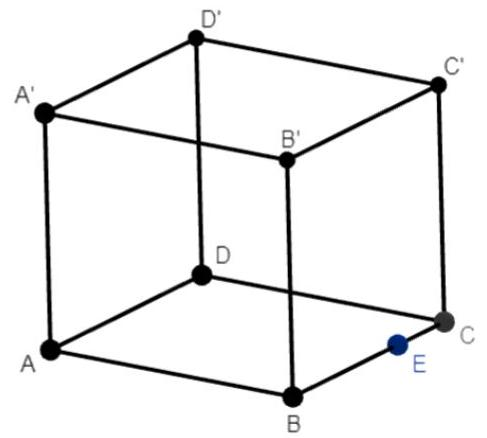
\includegraphics[max width=\textwidth, center]{2024_11_21_282fcc418c438279c74dg-1}\\
krawędzi podstawy. Na krawędzi BC wybrano taki punkt E, że \(|B E|:|E C|=2: 1\). Następnie punkty D' i E połączono odcinkiem o długości

\[
6 \sqrt{3}+\left(\frac{\sqrt[4]{3} \cdot 9 \cdot \sqrt[4]{9} \cdot \sqrt{27}}{81 \cdot \sqrt{\frac{1}{9}} \cdot \sqrt[4]{27}}\right)^{3} . \quad \text { Oblicz pole powierzchni }
\]

całkowitej tego graniastosłupa.

Zadanie 3. Dany jest trapez równoramienny, którego ramiona mają długość równą \(15+2,9\left(2,4-2 \frac{2}{5}\right)\). Wysokość równa \(\left(-\frac{12}{1,6}\right) \cdot\left(-1 \frac{3}{5}\right)\), opuszczona z wierzchołka kąta rozwartego, dzieli dłuższą podstawę w stosunku 1:3. Oblicz długości podstaw trapezu oraz jego pole.

Zadanie 4. Suma cyfr liczby trzycyfrowej jest równa 21. Jeżeli cyfrę setek zamienimy miejscami z cyfrą jedności to otrzymamy liczbę o 198 mniejszą od szukanej liczby. Znajdź tę liczbę wiedząc, że cyfra dziesiątek jest średnią arytmetyczną cyfry setek i jedności.

Zadanie 5. Wykaż, że iloczyn trzech kolejnych liczb podzielnych przez 6 dzieli się przez 1296.


\end{document}